\documentclass[prl,twocolumn,superscriptaddress,floatfix]{revtex4}
\usepackage[utf8]{inputenc}
\usepackage{graphicx}
\usepackage{float}
\usepackage{amsmath,amssymb,amstext}

% get rid of hbox badness 10000 in bbl file
\usepackage{etoolbox}
\apptocmd{\sloppy}{\hbadness 10000\relax}{}{}

\begin{document}

\title{Analysis of the Fourier Transformation and its Applications}
\author{Junseo Shin}
\affiliation{Department of Physics, Washington University, St.\ Louis, Missouri 63130}
\author{Jeremy Smith}
\affiliation{Department of Physics, Washington University, St.\ Louis, Missouri 63130}

\date{\today}

\begin{abstract}
The Fourier Transform converts a signal---e.g. AC or radio waves---initially presented in the time domain into the frequency domain.
Decomposing a signal into its constituent frequencies allows more information content to be extracted from a signal. 
Thus the Fourier Transform becomes a powerful tool in signal processing and analysis.
% Modern technology, such as the Stanford Research Systems SR770, 
Furthermore, the Fast Fourier Transform (FFT) is a 
a numerical algorithm that computes the Discrete Fourier Transform (DFT) of a sequence (or continuous signal) in rapid time---i.e. it reduces the computational complexity of a time series from $O(n^2)$ to $O(n \log n)$\cite{FFT}.
Although FFT allows for extremely fast and efficient frequency domain representation, there are limitations regarding the resolution of the frequency domain,
its sensitivity to noise, and spectral leakage. 
Here we show how FFT can be used for finding signals amongst noise, tuning into AM radio, and identifying properties of the fluxgate magnetometer. 
Fourier Transformations present a new set of tools for understanding how a signal behaves in the frequency domain.
We deciphered information in a particular signal by utilizing spectral density, harmonic analysis, and an rf (radio frequency) receiver module. 
From the three experiments, the analysis paradigm was rendered impossible in the time domain but now becomes possible in the frequency domain.
We propose that these experimental explorations will capture the utility and importance of Fourier methods in signal processing and analysis.
Furthermore, an intuitive understanding of Fourier Transformations will reveal the hidden yet visible applications of Fourier methods in the modern world. 
\end{abstract}
\maketitle

\section{Introduction}
Famous mathematician and educator Gilbert Strang stated that the FFT is ``the most important numerical algorithm of our lifetime''\cite{strang}.
This was in 1994 before the invention of the iPhone, and only a year after the World Wide Web was released into public domain\cite{cernweb}.
Now every handheld device utilizes a Fourier Transform in some fashion, from the cellular networks \& WiFi signals that connect us to the internet to the software that processes the images we take. But first, we should understand what a Fourier Transform is before we can understand its applications:

The Fourier Transform, shown below, is an integral transform that takes the time series of a function/signal shown as $f(x)$ and outputs a function defined by frequency $\omega$. 
\begin{equation}
f(\omega) = \int_{-\infty}^{\infty} f(x)e^{-i2\pi \omega x}dx  \label{firstequation}
\end{equation}
In plain language this integral states that the Fourier Transform multiplies each value of $f(x)$ for its entire domain by the complex cycling function $f(x)e^{-i2\pi \omega x}$. Therefore, only the components of $f(x)$ that oscillate survive and don't fall to zero. This produces a function $f(\omega)$ that gives the prominence of a given frequency in a time series function. When this is display over the entire frequency domain or ``full span'', the frequency domain analogy of a time varying signal is produced.
This can be best visualized using an oscilloscope (TDS1012) which displays data in the time domain and a Stanford Research spectrum analyzer 770 (SR770) which displays the frequency domain.
Also, note that the SR770 uses FFT which splices the time series into discrete segments and efficiently computes the DFT at blazing speeds. These tools as well as a function generator and electronic modules provided
by Teach Spin are the main tools used in our exploration of the Fourier Transform.

\begin{figure}[H]
    \begin{center}
    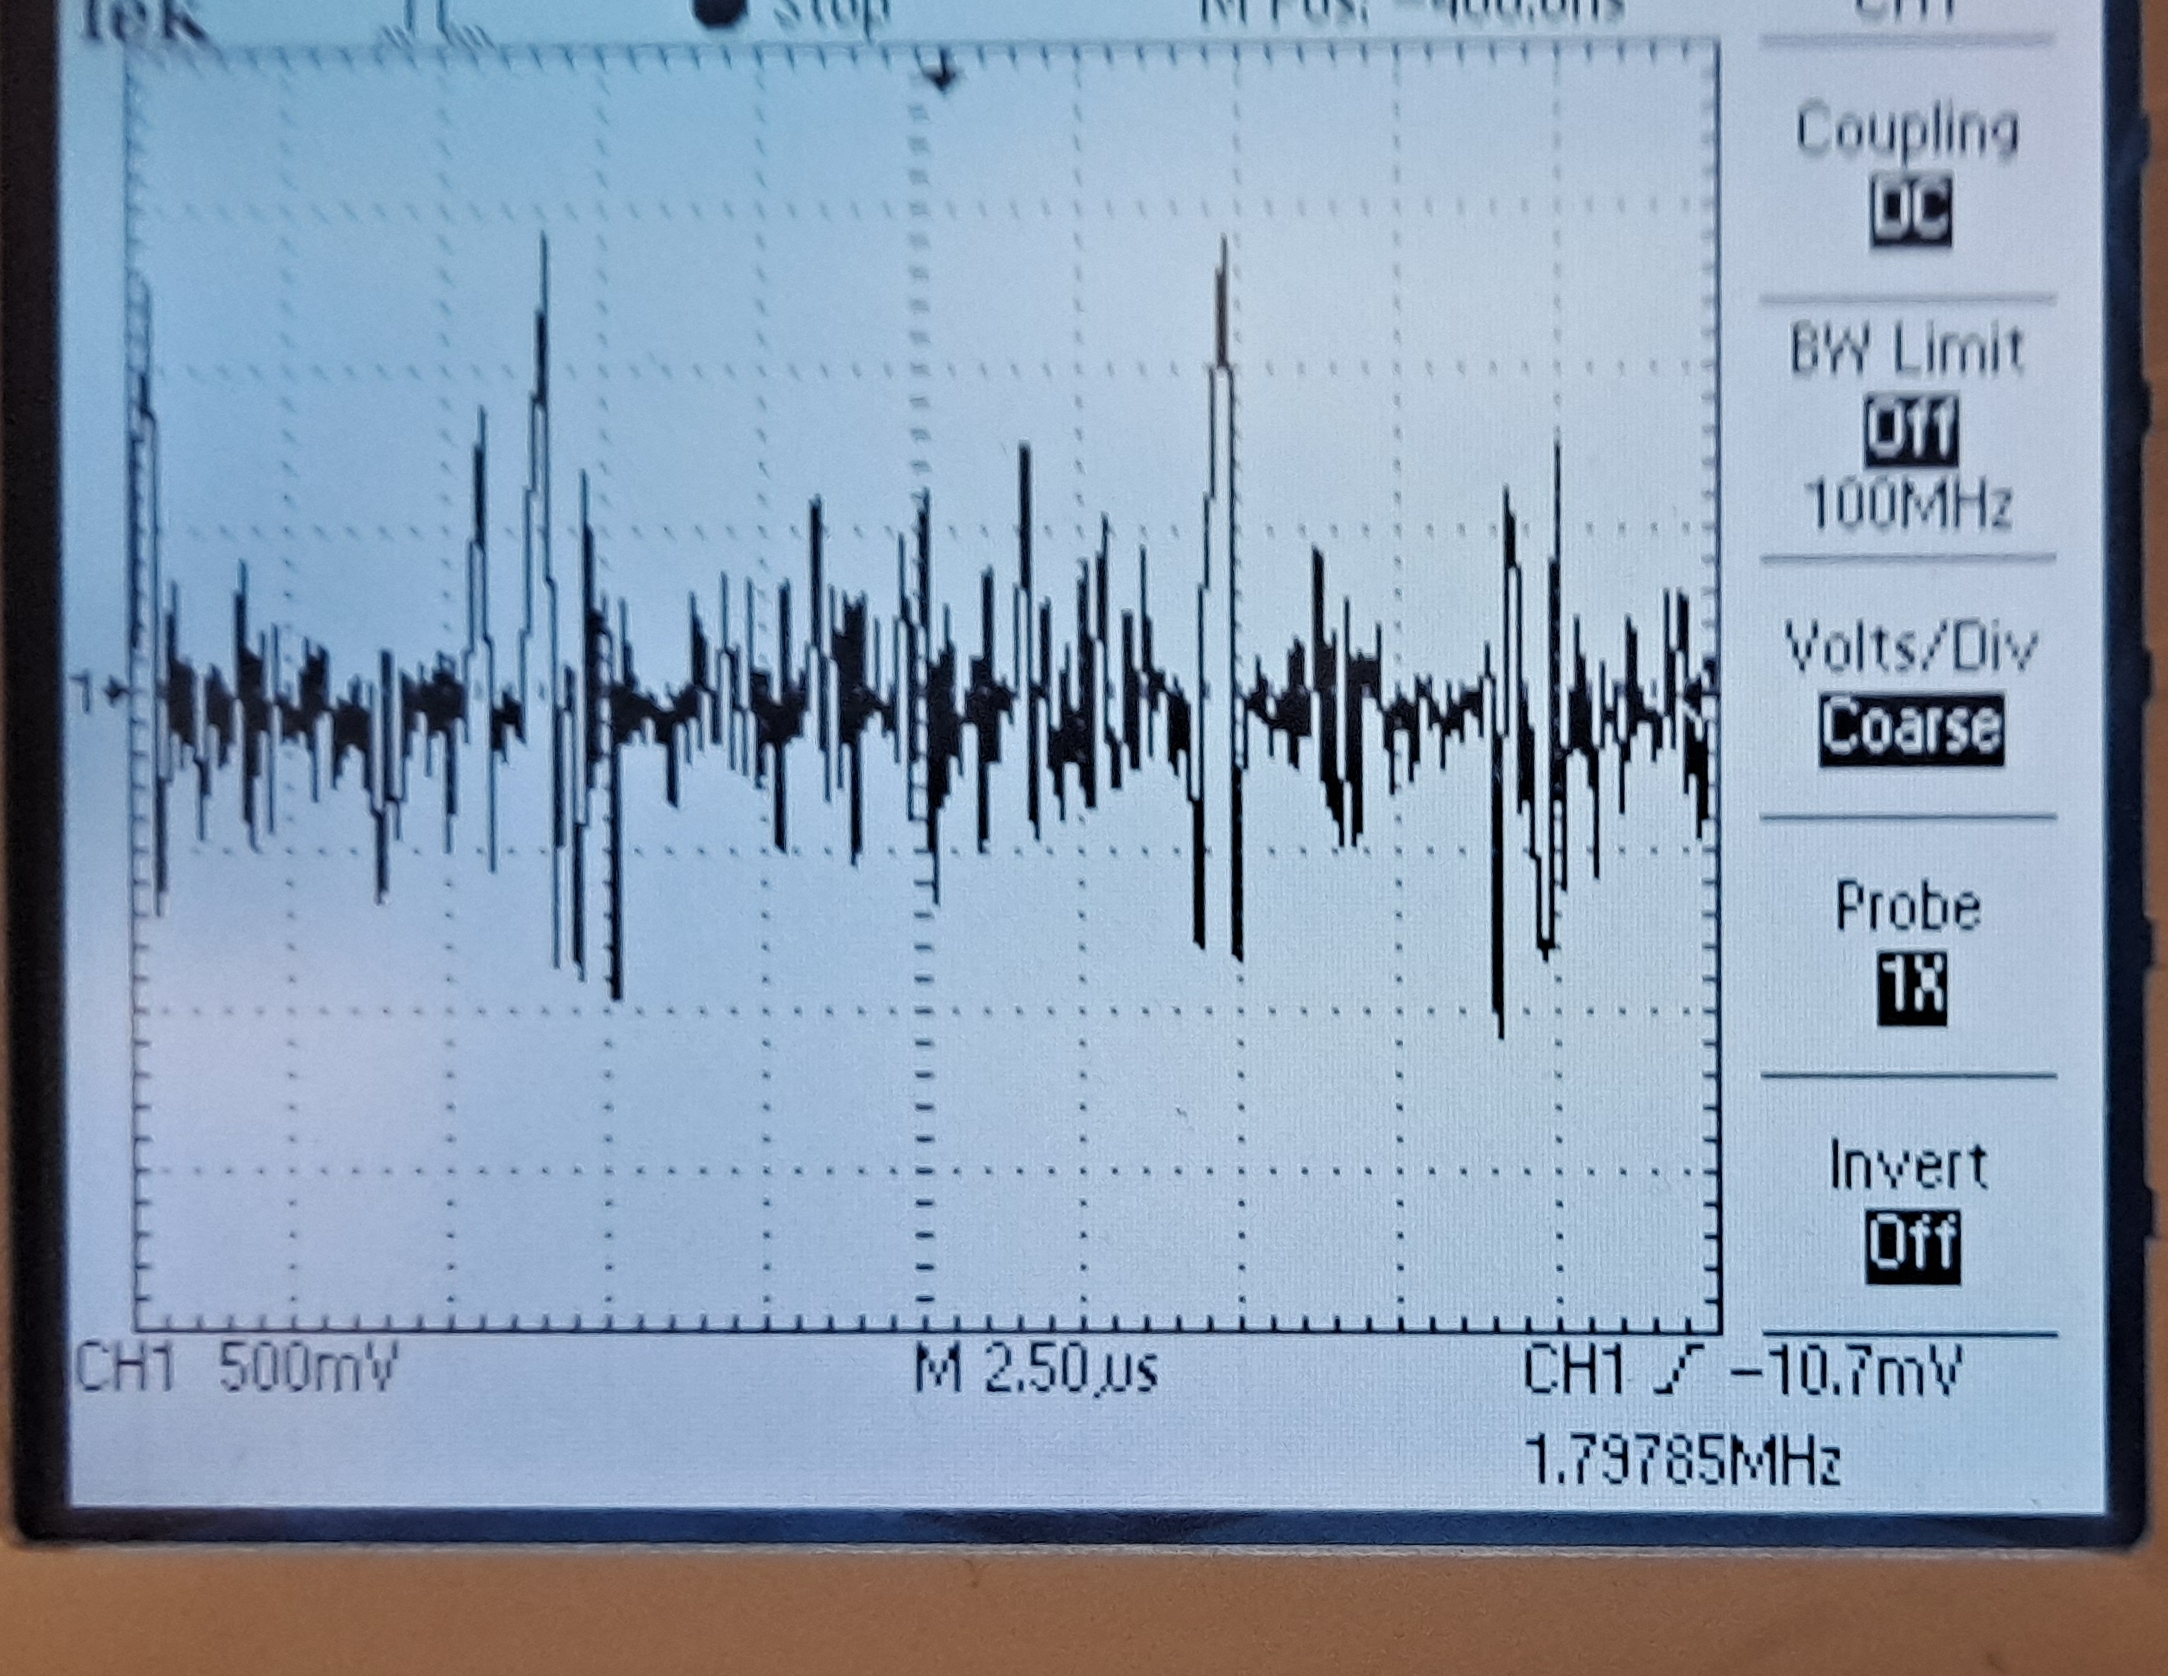
\includegraphics[width = 0.3\textwidth]{Time Data.jpg}
    \includegraphics[width = 0.3\textwidth]{Basic Sinusodial.jpg}
    \caption{\label{fig:1}Oscilloscope (top) and Spectrum Analyzer(bottom) view for a 50 kHz, 5 V sine wave superimposed with noise}
    \end{center}
\end{figure}

\section{Signal Recovery Under Noise} 
For our first experiment, we analyzed an unknown signal hidden under noise. Initially, as a proof of concept, we had a small amount of noise applied to a strong sinusoidal signal.
As shown in Fig. \ref{fig:1}, using the time domain approach (scope) demonstrates an interesting but indecipherable signal.
In the partnering image is the SR770 display in which it is almost impossible to miss the pure 50 kHz sine wave we inputted. 
We can also read the power of that individual signal itself. Due to the product of $f(x)$ and $e^{-i2 \pi \xi x}$, each frequency in the spectrum is displayed in a way that is proportional to its power.

One could, theoretically and with great difficulty, examine the time domain signal and derive the pure sinusoidal, but
becomes exceptionally difficult for a signal under much heavier noise as shown in Fig. \ref{fig:2}. 

\subsection{Methodology and Setup}
% figure of exp1_1.pdf
\begin{figure}[H]
    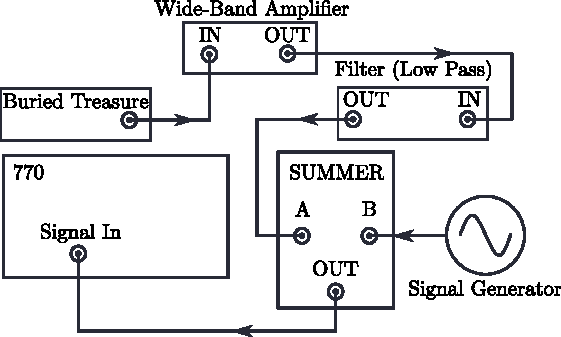
\includegraphics[width=0.45\textwidth]{exp1_1.pdf}
    \caption{Control setup for Signal Under Noise}
    \label{fig:exp1}
\end{figure}
Our first setup involved taking filtered noise from the buried treasure module and sending it through both an amplifier and a low-pass filter in order to generate a large amount of noise to hide a signal in. Then we superimposed a signal from our generator onto it using the summer module and is displayed on the SR770. This is all done in order to practice visually seeing what a signal amongst noise looks like on the SR770.
% figure of exp1_2.pdf
\begin{figure}[H]
    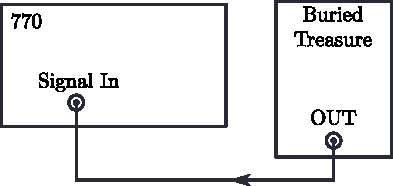
\includegraphics[width=0.45\textwidth]{exp1_2.pdf}
    \caption{Hidden Signal Under Noise from Buried Treasure}
    \label{fig:exp2}
\end{figure}
The next step was to locate a hidden signal of unknown frequency. We directly sent the C setting of the TeachSpin buried treasure module which consists of a noisy signal with a small pure sinusoidal waveform hidden in it to the SR770. We then utilized the Fourier transform via the SR770 to locate the waveform.
\begin{figure}[H]
    \begin{center}
    \includegraphics[width = 0.3\textwidth]{Time Data C.jpg}
    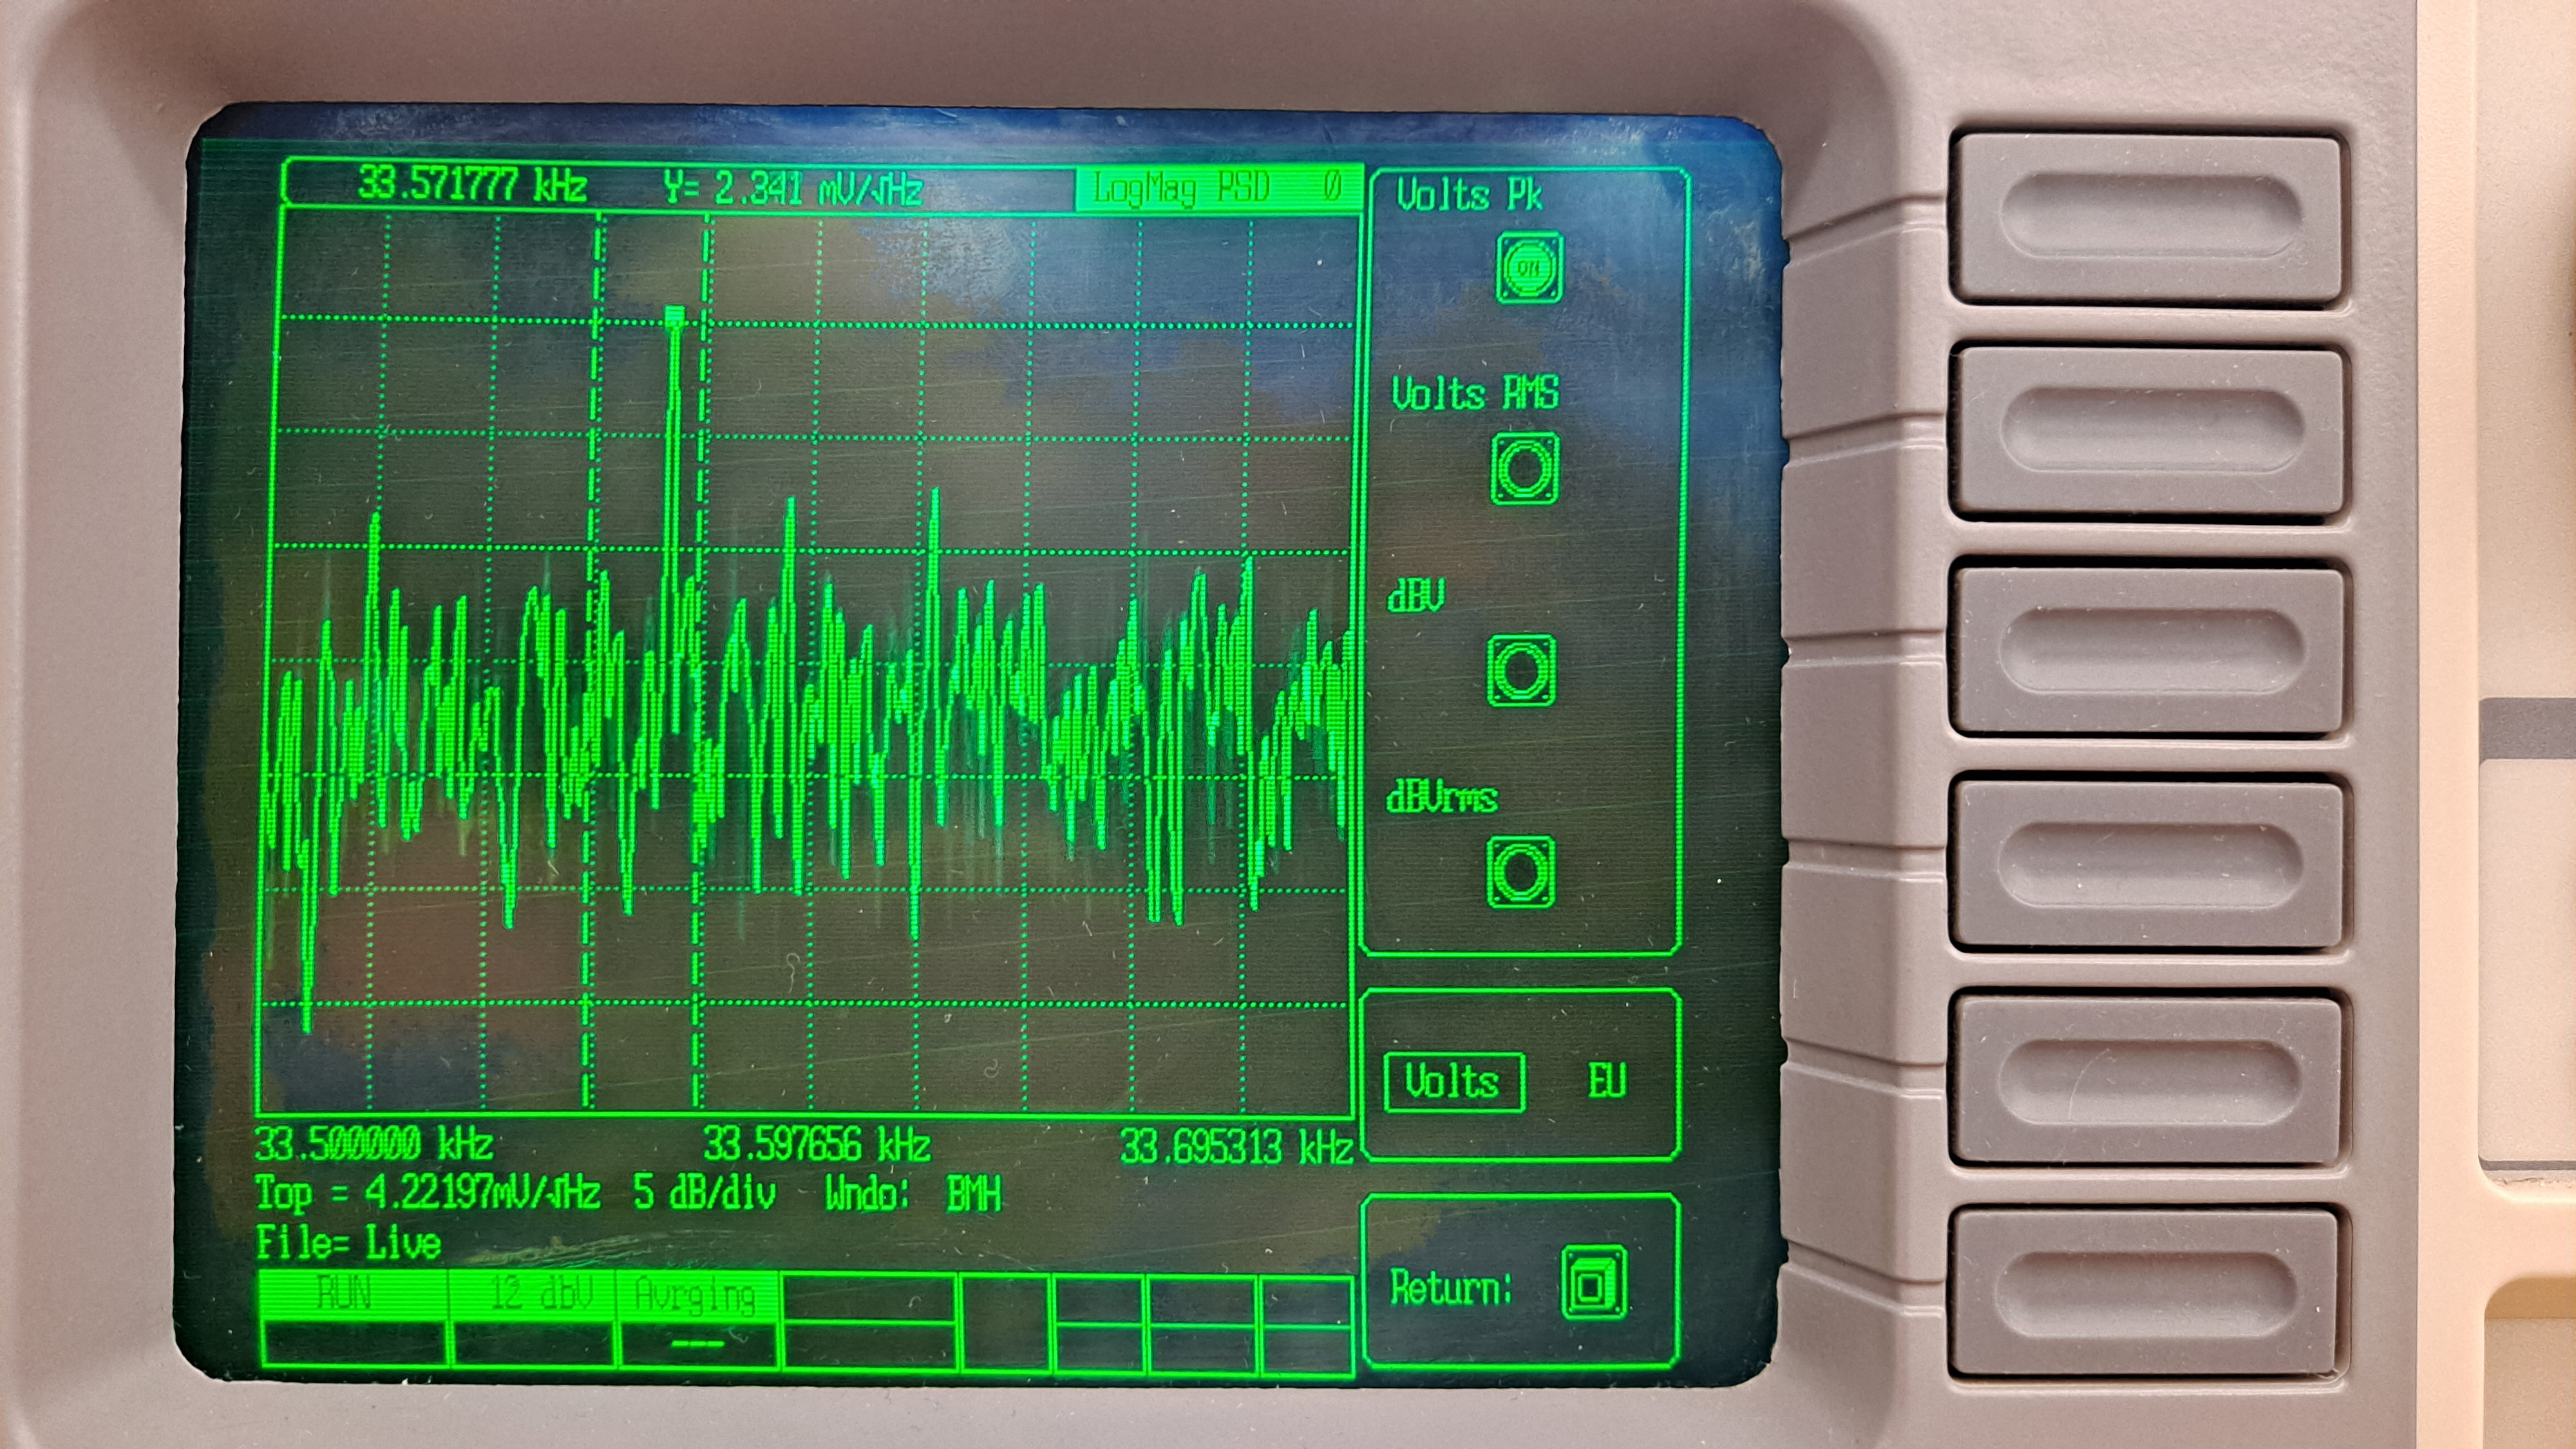
\includegraphics[width = 0.3\textwidth]{Signal C under Noise.jpg}
    \caption{\label{fig:2}Weak Signal under noise displayed in both the time and frequency domains.}
    \end{center}
\end{figure}

\subsection{Analysis}
In this time display it is much harder to understand the nature of the underlying pure waveform.
A much weaker waveform has been superimposed upon stronger noise.
Despite this, in the frequency domain, it is recoverable. So, how would one measure signal under noise?

Noise randomly sends power to each frequency with equal chance.
Therefore if one takes an average of noise over enough time, the averages should resolve to a flat uniform distribution in the frequency domain. As shown below in Fig. \ref{fig:averaged noise}

 \begin{figure}[H]
    \centering
    \includegraphics[width=0.3\textwidth]{Averaged Noise.jpg}
    \caption{Spectral Density of Noise}
    \label{fig:averaged noise}
 \end{figure}

Any interesting signal should be easily visible over the line as its average will vary from this.
Practically speaking, the SR770 takes its averages over a finite amount of time referred to as acquisition time.
Thus the process involved in identifying a weak signal among noise is presented as translating the signal to the frequency domain, taking sufficient averages, and using a fine enough span to visually spot it.
The act of taking those averages, however, is a process in itself. For a given noisy waveform, the amplitudes could be averages across a finite time span, our SR770 uses 4ms as the default, but since noise is statistically random, this would result in a 0 average, which is not useful. 
A better method would be to square the amplitudes first and then take the average, yielding the average power of the signal known as $V_{rms}$. 
We can then, in the frequency domain, divide by each frequency and get $V_{rms}/\sqrt{Hz}$. 
This new term we've derived, the voltage spectral density (VSD), is the actual value we read on the SR770 and displays each frequency by its respective power contribution. Correspondingly the square of this value is the power spectral density (PSD) which is directly proportional to the power contribution of noise.

The power of noise is continuously distributed across the spectrum when we measure spectral density, so we can now compare the power (or mean-square voltage) in noise to the power of a sinusoidal signal. Furthermore, averaging the measurements will decrease the magnitude of the spectral density from noise---i.e. lowering the noise floor---without affecting the magnitude of the spectral density from the sinusoidal signal. 
% to compare the power (or mean-square violate) in a noise signal to the power of a sinusodial signal we use the power spectral density to evaluate the power as it is distributed continuously on the spectrum

With the measure of spectral density, we can now recover the signal under noise as long as we chose a small enough frequency span and swept through the full span of 100 kHz until we found a visible signal peak. 
By default, this method of signal recovery is limited by the acquisition time,$T_{acq}$, required for a given frequency resolution,$f_\textrm{resolution}$, the SR770 i.e.
the frequency-duration ``uncertainty principle'' \cite{fouriermethods}
\begin{equation}
    f_\textrm{resolution} \cdot T_{acq} \geq \textbf{constant}
\end{equation}
This constant is a dimensionless magic number attached to the frequency-resolution condition on the SR770. For example,
the SR770 defines its magic number (with a default acquisition time of 4 ms for the full 100 kHz span)
to be $400$, so for a frequency span of 195 Hz shown in Fig \ref{fig:2} the acquisition time for a single measurement is $400 / 195 = 2$ s. In addition, averaging 64 measurements to decrease the spectral density of the noise floor adds computational time as well for each measurement. For example, we had to repeat this for roughly 170 measurements from 0 to 33.5 kHz as we swept across the full span until we found our small signal at 33.572 kHz shown in Fig. \ref{fig:2}.

\section{AM Radio Reception}

Beyond just detection, the Fourier Transform can be useful in analyzing the properties of waveforms as well.
In AM radio, program content $f_{p}$ consists of a variable signal which is the actual data, i.e. sound, and the product of that and a pure carrier frequency $f_{c}$ creates an amplitude-modulated signal containing program data.
This can be formulated as the equation:
\begin{equation}
    V(t) = A[cos(2\pi f_{c}t)+0.5cos(2\pi(f_{c} \pm f_{p})t)]
\end{equation}
where A is the fixed amplitude of the carrier frequency.
This shows what an amplitude-modulated wave is, a central carrier frequency with a varying program frequency superimposed on it, and the variations in the 2nd term aka the program frequency, contain the data and content of the signal.
This allows a higher frequency wave which has a better time propagating across space to ``carry'' a small program wave.
Then at the receiver one simply has to use a local oscillator to ``tune'' to a specific carrier wave and then demodulate by filtering out that carrier, leaving only the program content.
\subsection{Methodology and Setup}
\begin{figure}[H]
    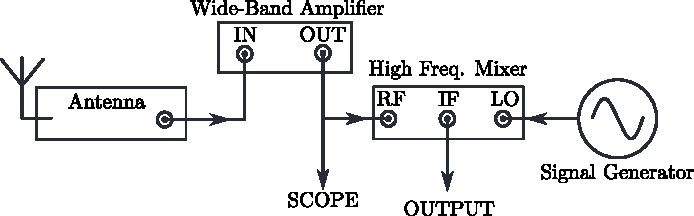
\includegraphics[width=0.45\textwidth]{exp2_1.pdf}
    \caption{Experimental setup for AM radio reception Part I}
    \label{fig:AM1}
\end{figure}
For the amplitude modulation we connected an antenna with a built in impedance adjuster, after amplifying it, to our scope in order to help visualize the signal. We also took this and mixed it with a signal from our waveform generator using the TeachSpin's Frequency mixer. This allowed the waveform generator to act as a local oscillator and tune into the desired carrier frequency. After which the mixer extracts the program content from the carrier signal. 
\begin{figure}[H]
    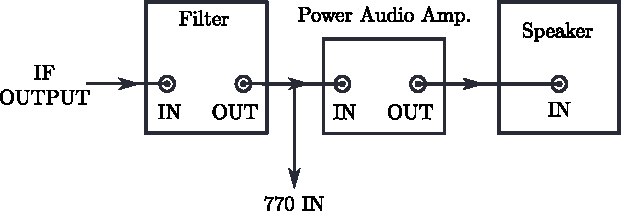
\includegraphics[width=0.45\textwidth]{exp2_2.pdf}
    \caption{Experimental setup for AM radio reception Part II}
    \label{fig:AM2}
\end{figure}
Finally we boosted the processed signal with an audio amplifier and connected it to a speaker in order to actually hear the AM radio station we were tuned into.
The first image in Fig 4 shows an example we generated, with the full signal above and the carrier sinusoidal below.

\subsection{Analysis}
\begin{figure}[H]
\begin{center}
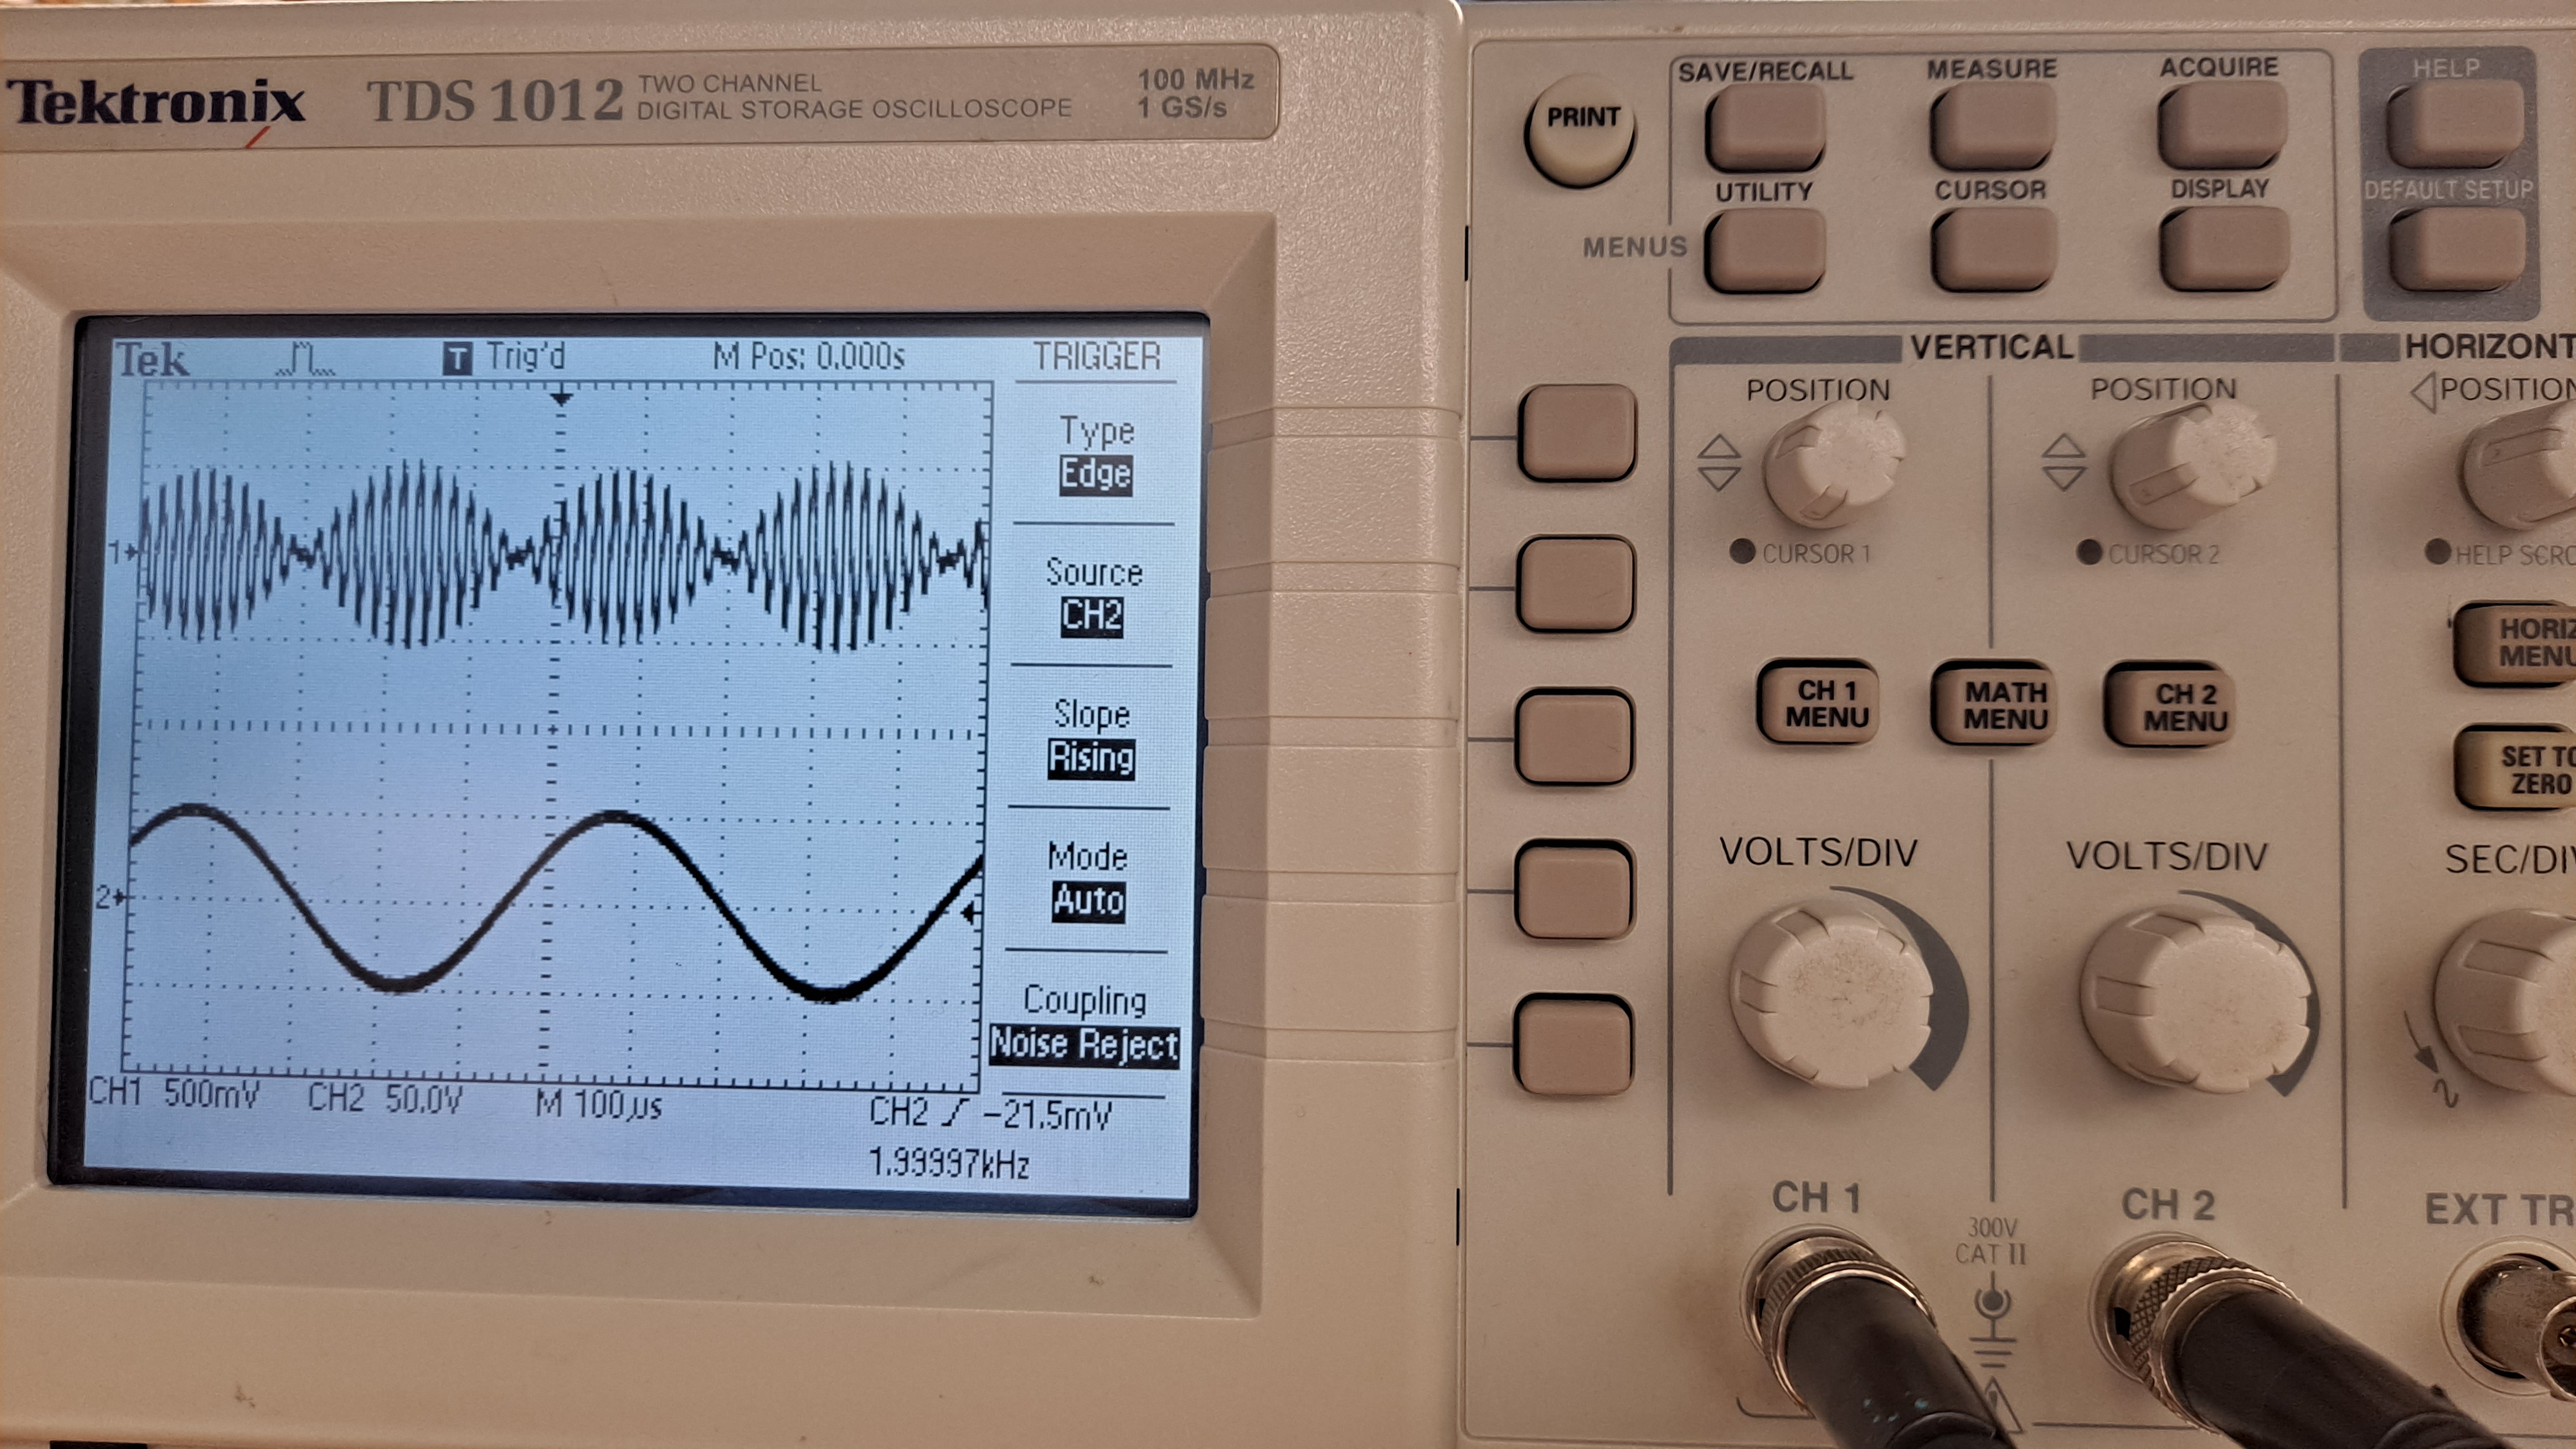
\includegraphics[width = 0.3\textwidth]{AM data, Time.jpg}
\end{center}
\end{figure}
\begin{figure}[H]
\begin{center}
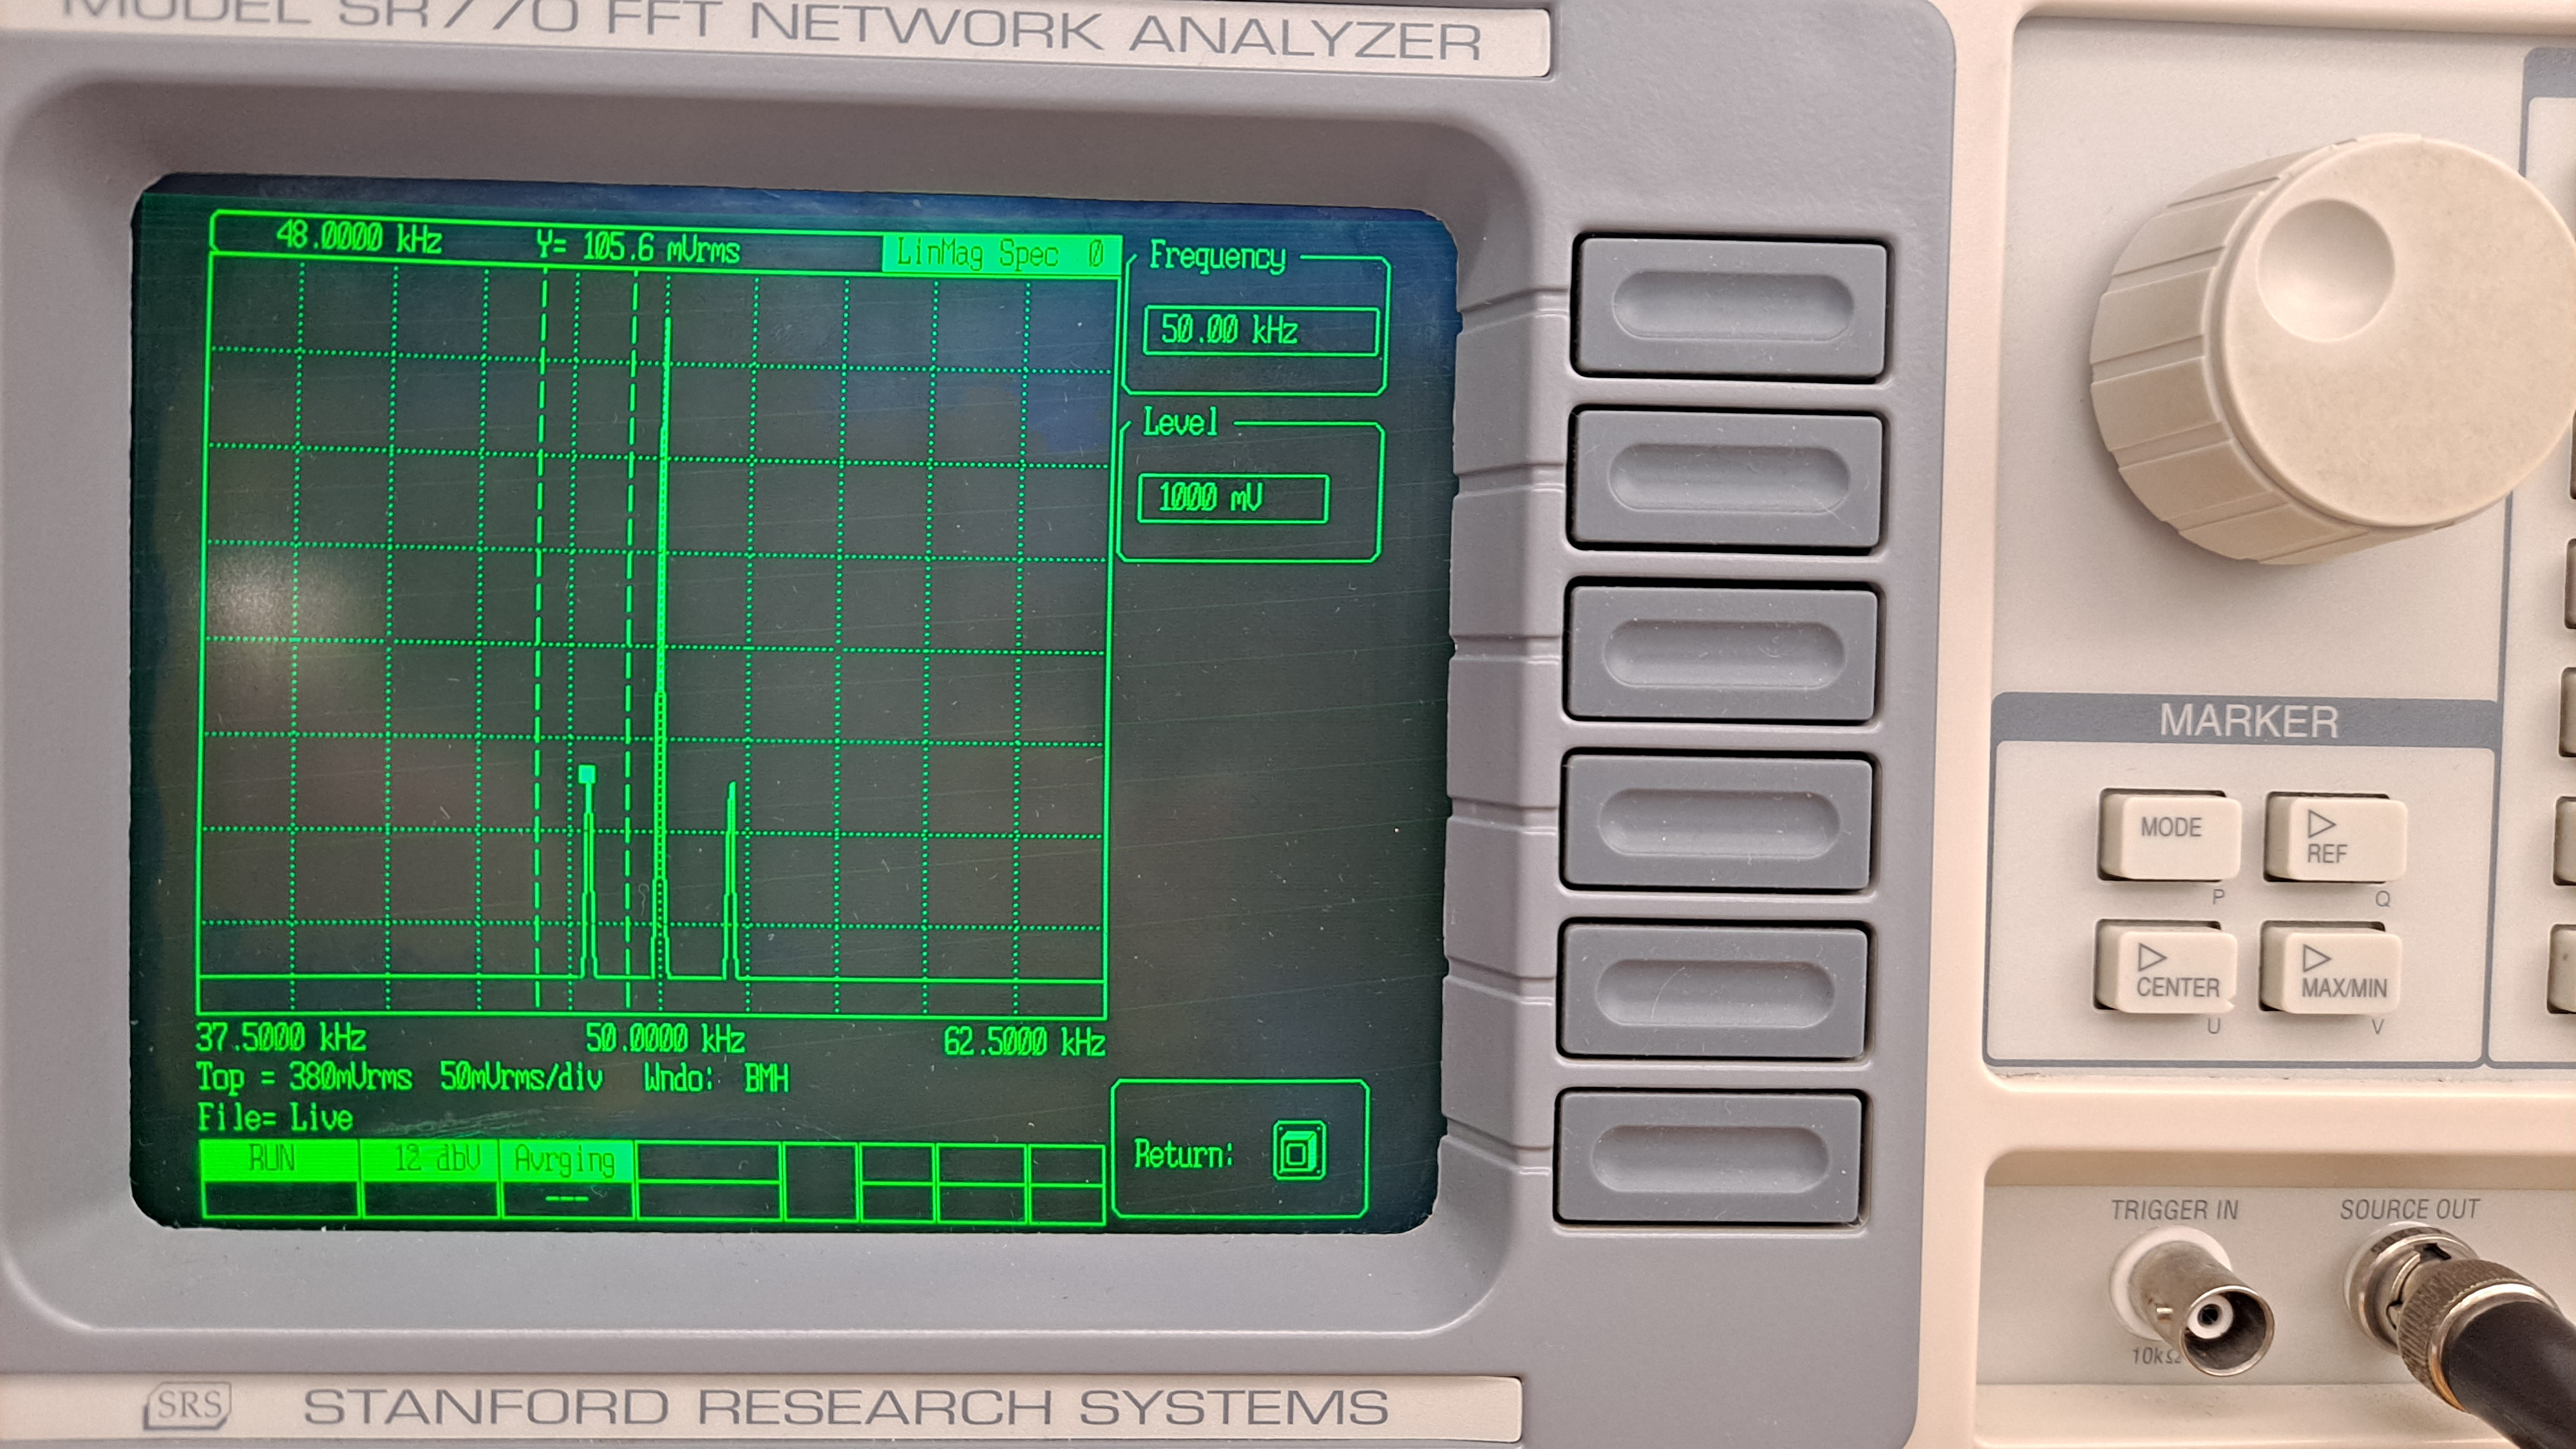
\includegraphics[width = 0.3\textwidth]{AM data, Freq.jpg}
\caption{\label{amfreq}Amplitude modulated signal in both domains.}
\end{center}
\end{figure}
After setup we were able to capture the data from a local AM radio station in the time domain as shown in Fig \ref{amfreq}. This is a fairly interesting signal, however, just like in the previous case, we can only gain so much information from this.
Moving to the frequency domain, we can better see the properties of the signal, The central peak is the carrier wave and the side bands demonstrate program content.
This allows us to better view the entire AM spectrum. If there are, as there are in real applications, numerous radio sources all broadcasting in space, how would our devices tune to the one we desire without this methodology?
Using Fourier Transformations and the frequency domain we can see each station and the program content is represented by the sidebands on either side. 

\section{The Fluxgate Magnetometer}

Our third attempt at utilizing the Fourier methodology involves magnetic fields. 
In our next experiment, we examined how the Fourier Transform could be used with a magnetometer to ascertain the information content of magnetic fields.
The fluxgate magnetometer is a sensor made up of a ferromagnetic core---specifically ferrite material to reduce eddy current loss---wrapped by a primary driving coil and secondary pickup coil. The driving coil sends an AC to the solenoid which generates an AC magnetic field. As the fluxgate sensor is subject to an external magnetic field, the generated emf is picked up by the secondary coil as an AC signal. The Fourier decomposition of this AC signal contains a 2nd harmonic component in response to the magnetization of the ferromagnetic core which is highly sensitive to an external magnetic field.

\subsection{Methodology and Setup}
\begin{figure}[H]
    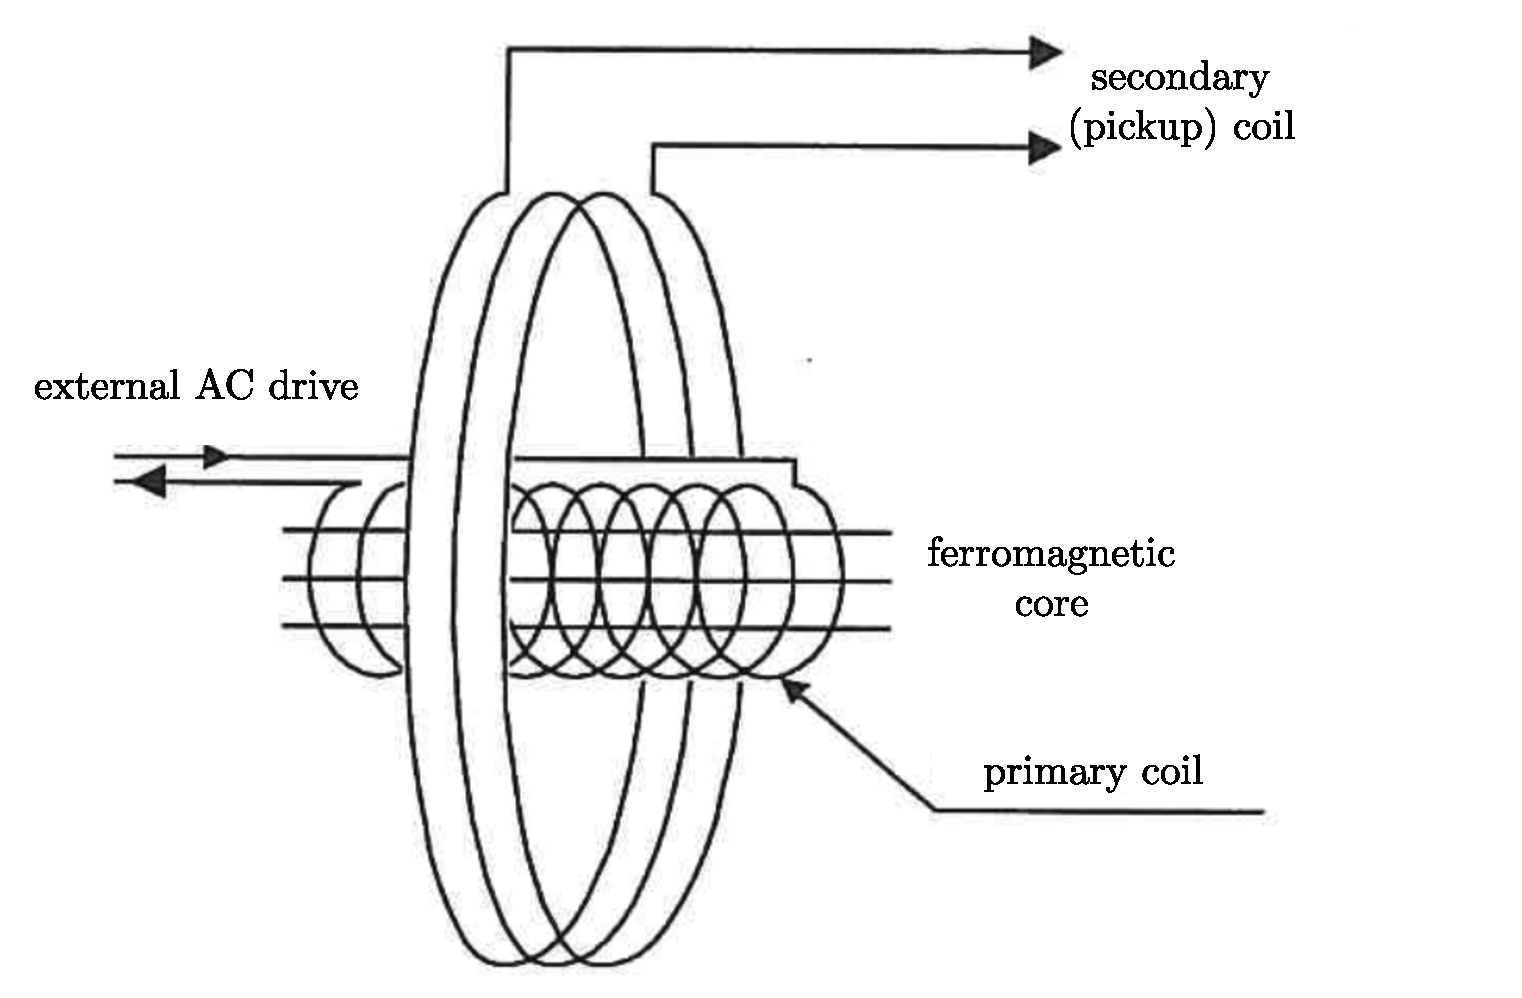
\includegraphics[width=0.45\textwidth]{exp3_1.pdf}
    \caption{Simplified Fluxgagte Magnetometer}
    \label{fig:fluxgate}
\end{figure}

\begin{figure}[H]
    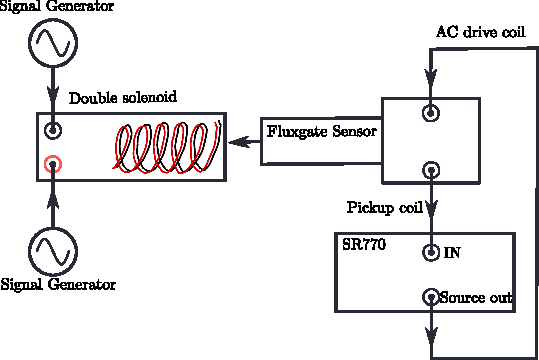
\includegraphics[width=0.45\textwidth]{exp3_2.pdf}
    \caption{Double coil apparatus with Fluxgate (magnetometer) Sensor}
    \label{fig:doublecoil}
\end{figure}
Fluxgate Magnetometers work by sending a known AC through the AC drive coil inducing a magnetization within the iron core. Due to hysteresis there is a lag between the change in the magnetic field produced in the coil and the one produced by the magnetization of the core. This causes the core field and the AC coil field to cancel out. In the presence of an external field however, the iron core experiences a magnetization not equal to the AC drive and therefore a net magnetic field is produced by the whole system. Via induction this produces a current within the secondary pickup coil and this is the actual sensor signal. 

\begin{figure}[H]
    \begin{center}
    \includegraphics[width = 0.3\textwidth]{fig11a.jpg}
    \includegraphics[width = 0.3\textwidth]{fig11b.jpg}
    \caption{\label{fig:11} (Top) 770 view of one AC magnetic field and (Bottom) two AC magnetic fields}
    \end{center}
\end{figure}
\subsection{Analysis}

In the experiment, the fluxgate magnetometer was able to detect external magnetic fields of the Earth and isolate multiple AC magnetic fields being detected by the fluxgate sensor using the SR770 as shown in Fig. \ref{fig:11}. Moreover, the fluxgate sensor becomes a real-time AC-field spectrometer that is highly sensitive to magnetic fields and low AC frequencies.
Later on, we noticed that the fluxgate sensor was also affected by the magnetic fields produced by the nearby pulsed NMR machine which contains a 1.4 T or 2.1 T permanent magnet whereas the Earth's magnetic field on the surface is in the order of $\mu T$ \cite{Cornell2000}.

<<<<<<< HEAD
\begin{figure}[H]
    \centering
    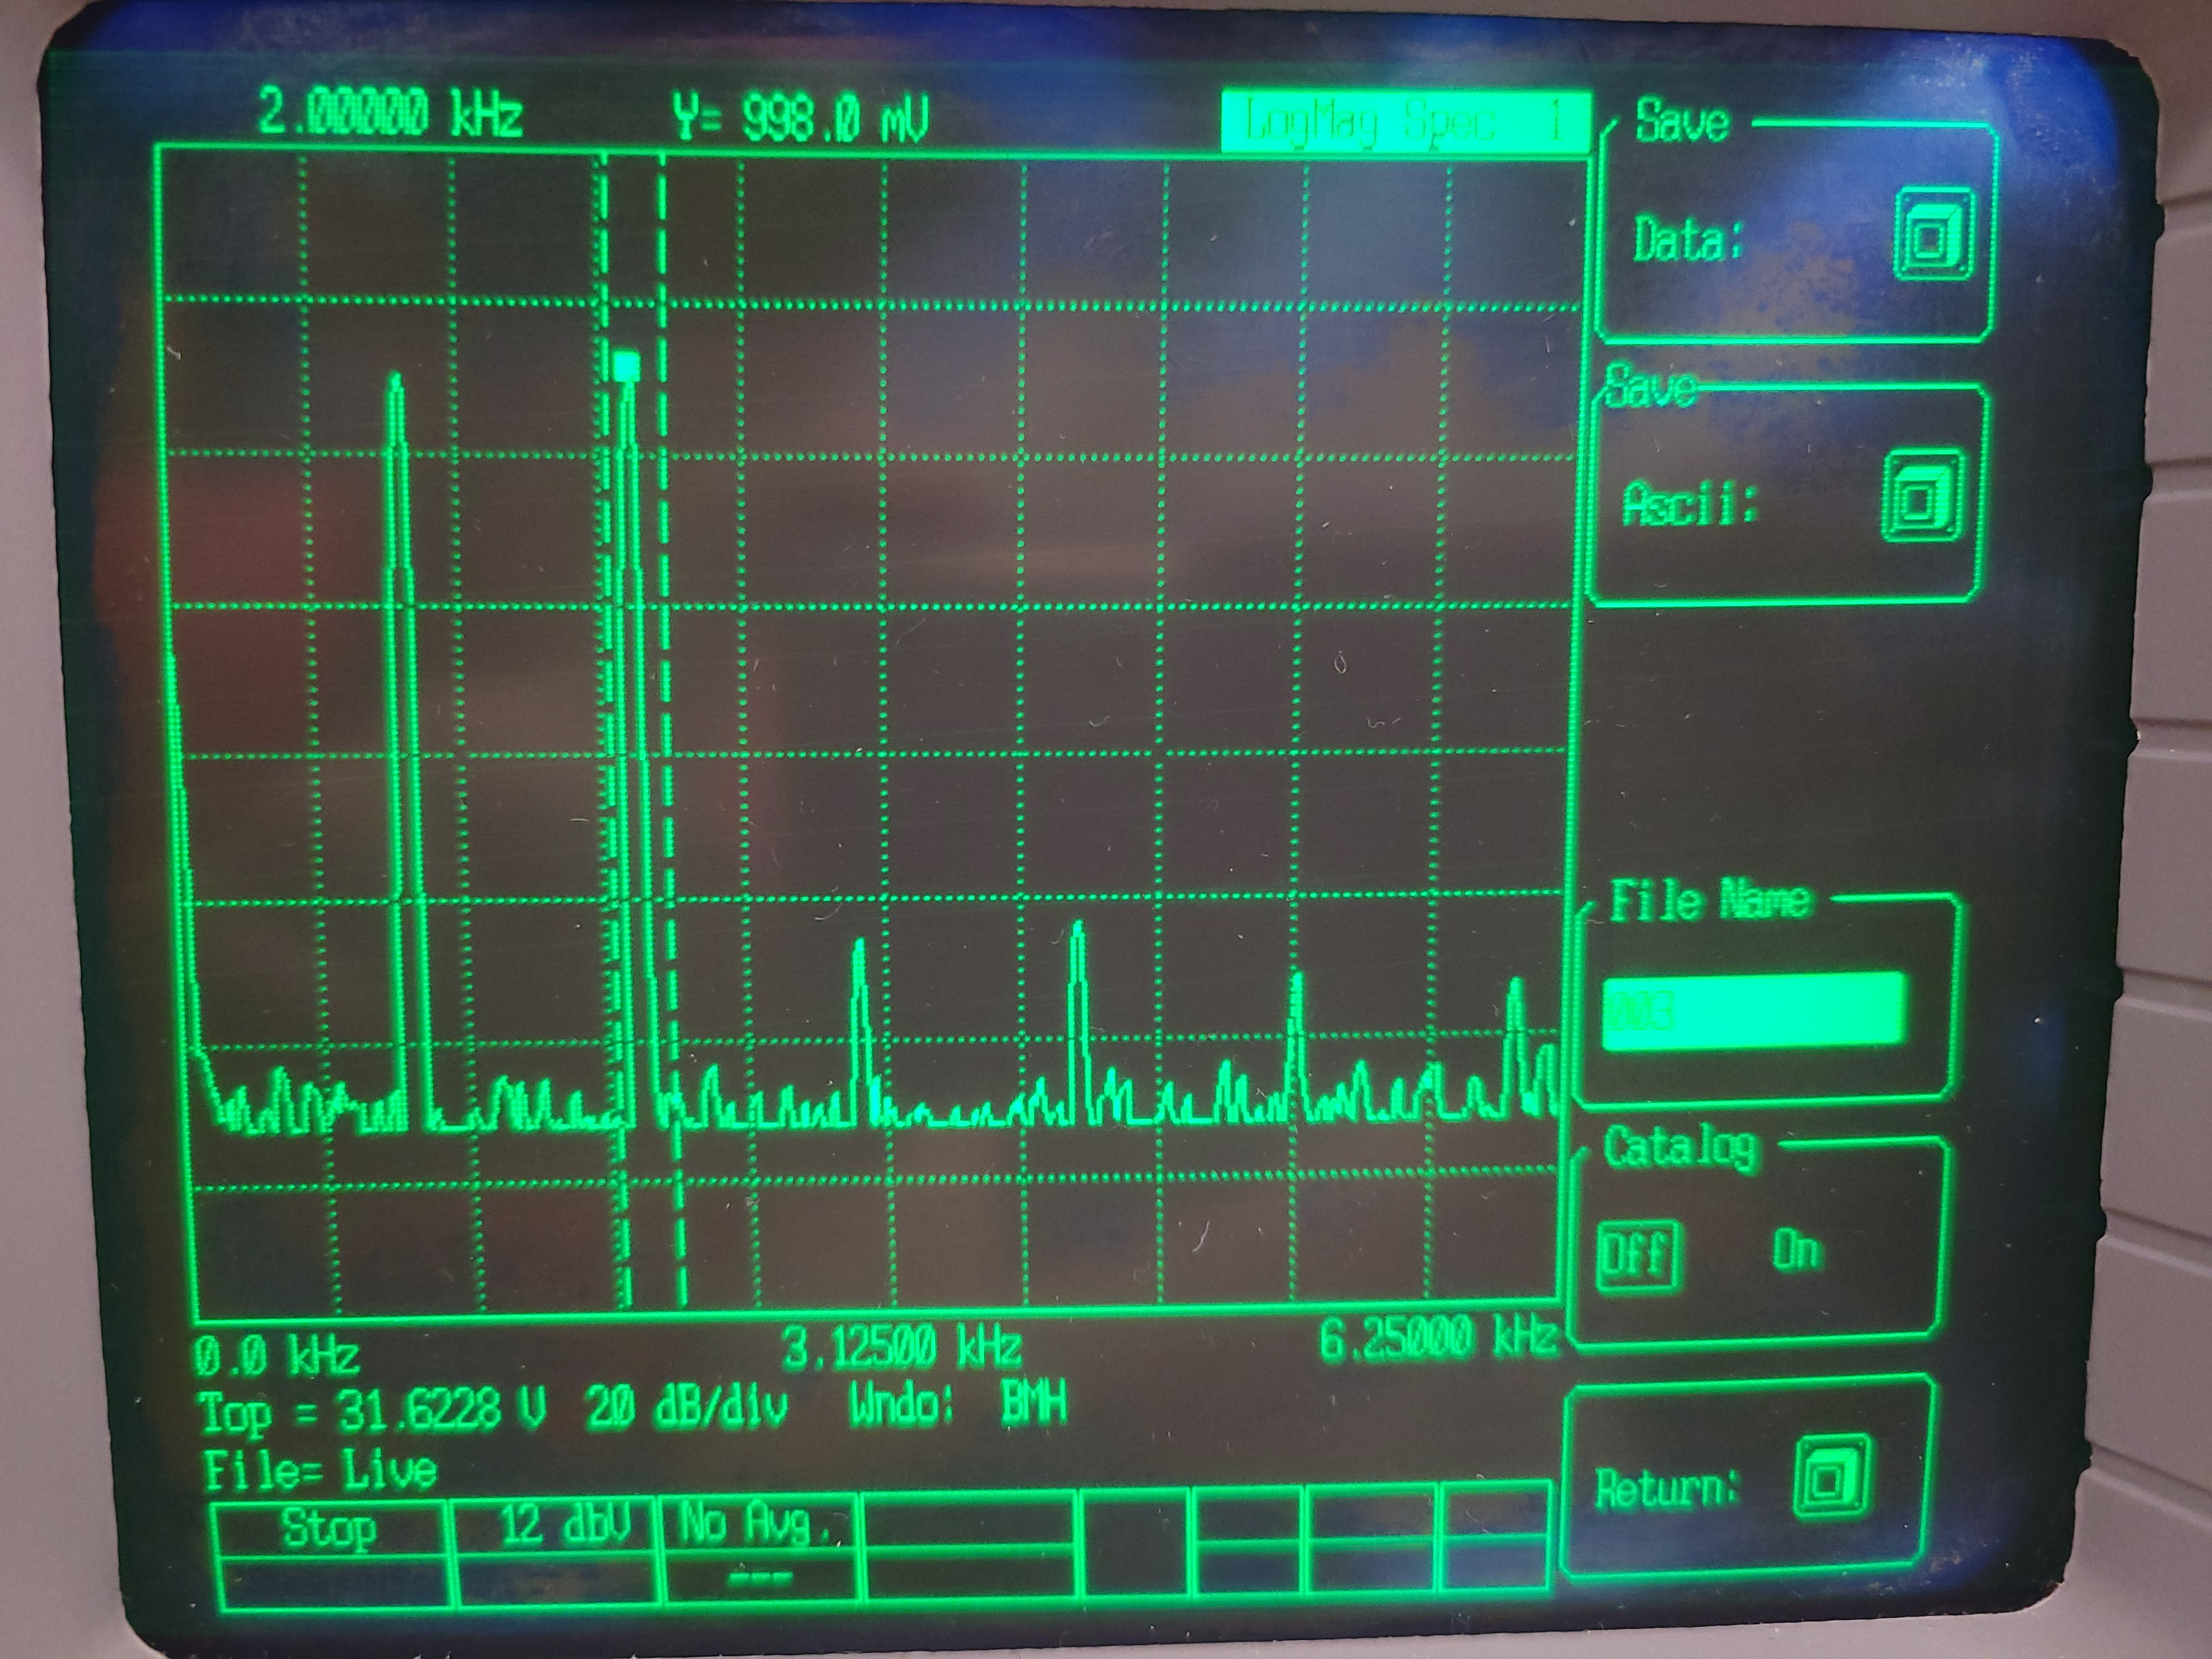
\includegraphics[width=0.3\textwidth]{Magnetometer Data.jpg}
    \caption{The harmonics of the Magnetometer}
    \label{fig:enter-label}
\end{figure}

\section{Methods}

% figure of exp1_1.pdf
\begin{figure}[H]
    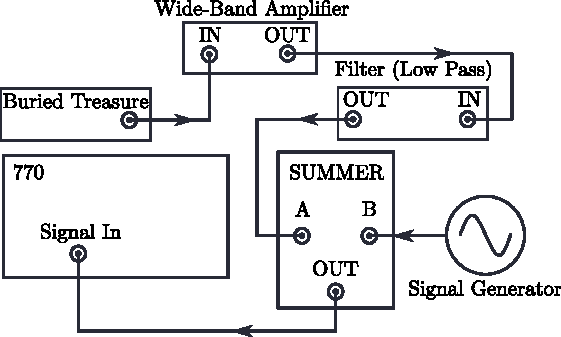
\includegraphics[width=0.45\textwidth]{exp1_1.pdf}
    \caption{Control setup for Signal Under Noise}
    \label{fig:exp1}
\end{figure}
[insert explanation]
% figure of exp1_2.pdf
\begin{figure}[H]
    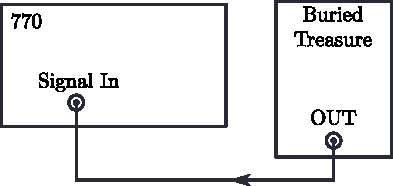
\includegraphics[width=0.45\textwidth]{exp1_2.pdf}
    \caption{Hidden Signal Under Noise from Buried Treasure}
    \label{fig:exp2}
\end{figure}
[insert explanation]
\begin{figure}[H]
    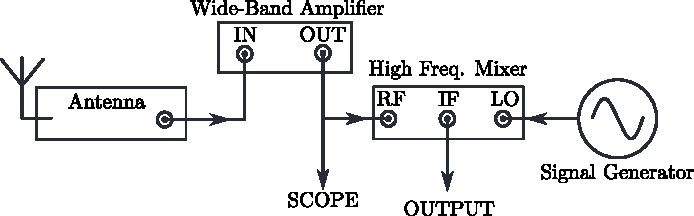
\includegraphics[width=0.45\textwidth]{exp2_1.pdf}
    \caption{Experimental setup for AM radio reception Part I}
    \label{fig:AM1}
\end{figure}
[insert explanation]
\begin{figure}[H]
    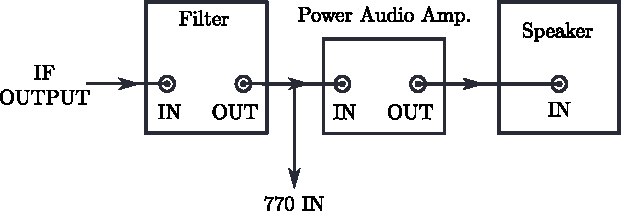
\includegraphics[width=0.45\textwidth]{exp2_2.pdf}
    \caption{Experimental setup for AM radio reception Part II}
    \label{fig:AM2}
\end{figure}
[insert explanation]
\begin{figure}[H]
    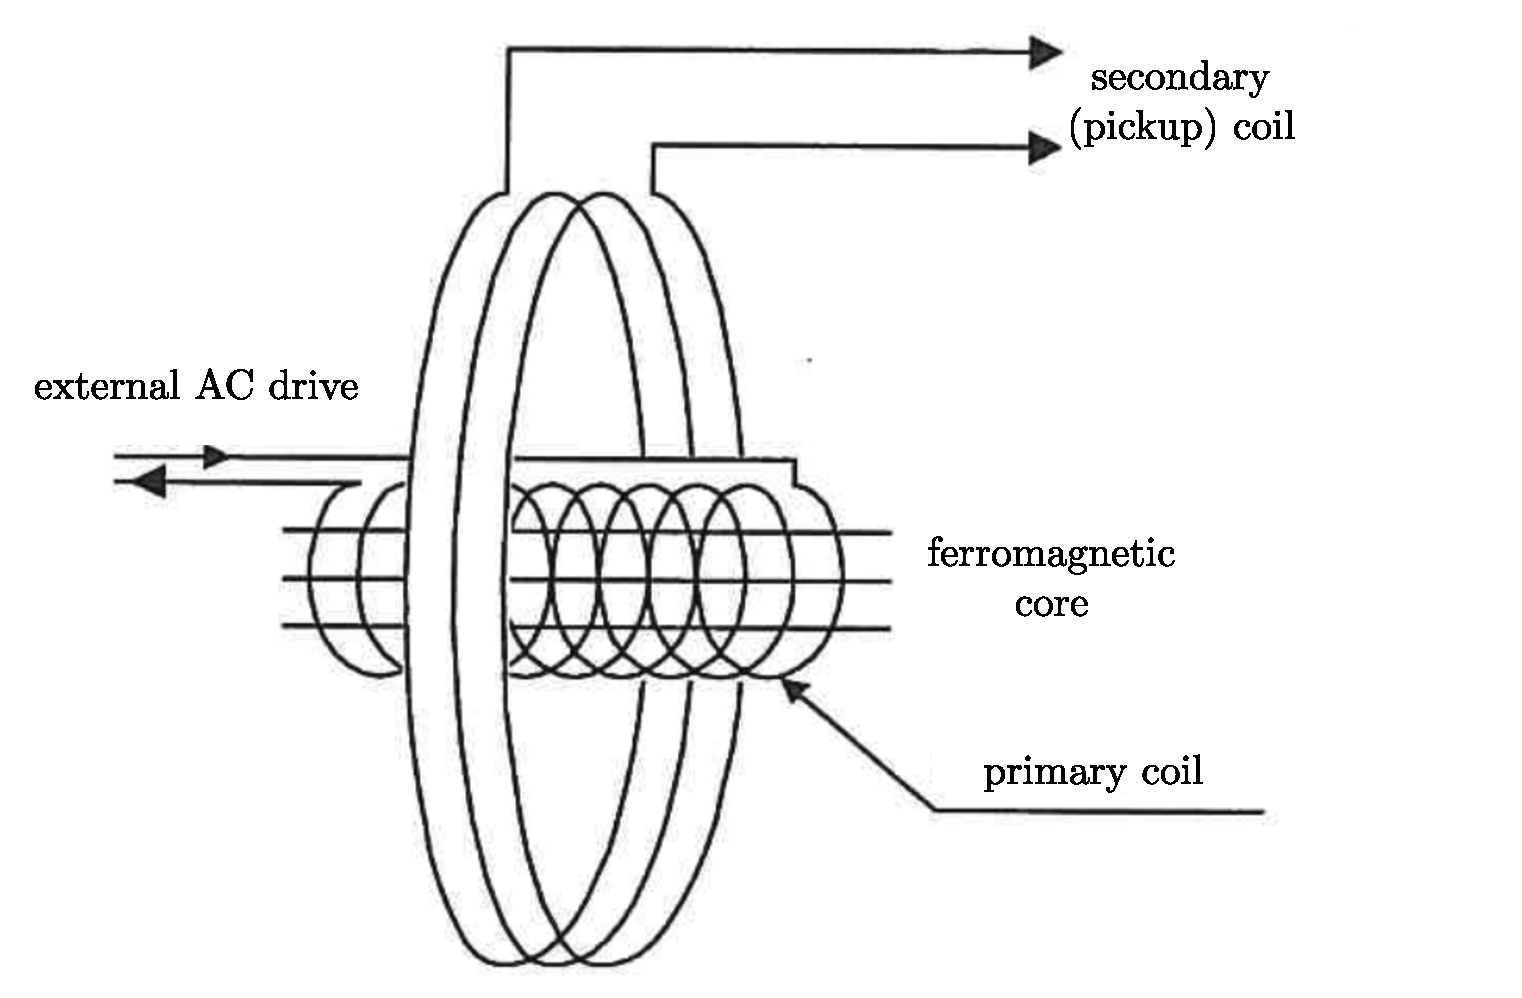
\includegraphics[width=0.45\textwidth]{exp3_1.pdf}
    \caption{Simplified Fluxgagte Magnetometer}
    \label{fig:fluxgate}
\end{figure}
[insert explanation of fluxgate magnetometer]

[insert diagram for setup with double coil]

[insert explanation]
\section{Conclusion}
=======
  \section{Conclusion}
The Fourier transform is a mathematical operation that dissolves a complex and potentially indecipherable signal into its frequency components. Done by displaying the product of the time series data and an oscillating mathematical function over the entire frequency span. We've shown this methodology to be useful in signal detection, wave modulation, and sensor data. Any signal with oscillating components, from radio telescope data to audio data, should reveal new properties and insights into the data. 
>>>>>>> eed00c4 (plan)
Hopefully, the varied nature of our application and analyses will motivate the reader that the Fourier Transformation is a useful lens for any signal analysis.
Viewing signals by their frequency domain should be, in the minds of these authors, a fundamental aspect of data collection.

\nocite{Butz2015}
\bibliography{myrefs}

\end{document}